\chapter{Related work}
\label{c:relatedwork}

\todo[inline]{Introductory Paragraph}

\section[Trace-Based Visualization of Object Interactions]{Trace-Based Visualization of Object Interactions%
\sectionmark{Trace Visualizations}}
\sectionmark{Trace Visualizations}

De Pauw et al. present a number of object-oriented views \cite{de_pauw_visualizing_1993, tokoro_modeling_1994} that can be generated and updated either live during the execution of instrumented code or post-mortem from recorded execution traces.
In our context of object interactions, the \emph{Functions-Instances Matrix} view  which shows the number of calls of specific methods on specific instances is of particular interest (cf. Figure \ref{fig:NotationInteractionMatrix}).
Methods are drawn on the y axis and instances are shown on the x axis.
Each box in the matrix denotes a call of the method from the left on the object at the bottom.
The color of the box indicates the number of invocations.
Although the diagram doesn't show object interactions in the presented form, it could be easily extended in this sense by replacing the static information on the y axis that abstracts from concrete instances through corresponding representations.
However, this matrix can not be utilized to visualize a specific sequence of function invocations or the state of the instances, both of which are important concepts of \textsc{PathObjects}.
The other presented views mainly focus on classes and their relationships, but an adaption to a visualization at the abstraction level of objects is straightforward in most cases.

DePauw et al. also propose a derivative of Jacobson's interaction diagrams \cite{de_pauw_execution_1998, jacobson_object-oriented_2004} that has been incorporated into \textsc{Ovation} \cite{de_pauw_visualizing_1993, tokoro_modeling_1994} and \textsc{Jinsight} \cite{de_pauw_visualizing_1998}.
The so-called execution pattern notation (cf. Figure \ref{fig:NotationExecutionPattern}) resembles a horizontal tree structure and adopts the concepts of displaying active objects as vertical boxes and of using straight arrows to represent message sends between objects.
But in contrast to Jacobson's proposal, there is no one-to-one mapping of objects and rails (the vertical lines in a diagram), since arrows are drawn strictly from left to right and top to bottom.
Therefor, each object has to be allowed to appear multiple times in a diagram, as otherwise it would be impossible to depict all object interactions, particularly message sends from objects that appear in lower hirarchies of the tree structure to objects of higher hirarchies (e.g. the call from object B to object A in Figure \ref{fig:06-1-DePauw}).
In their interactive implementation that allows to expand and collapse sub-trees, the objects' classes are illustrated through different colors and objects are labeled with an integer identifier.
The authors favor this concept over directed graphs since the latter do not inherently offer a notation of time and sequence (a problem that \textsc{PathObjects} solves through interactivity).
They further argue that compared to Jacobson's notation, their approach decreases clutter and increases readability while at the same time reducing the required space to depict object interactions.

\begin{figure}[tb]
	\centering
	
	\begin{subfigure}[b]{0.45\textwidth}
		\centering
        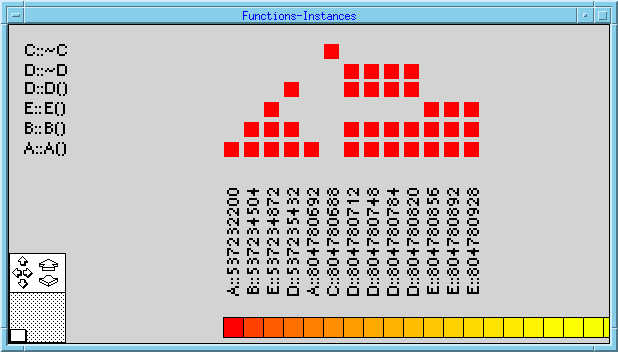
\includegraphics[width=\textwidth]{../images/06-DePauw-Matrix}
        \caption[Functions-Instances-Matrix by de Pauw et al.]{}
		\label{fig:NotationInteractionMatrix}
	\end{subfigure}
	\quad
	\begin{subfigure}[b]{0.45\textwidth}
		\centering
		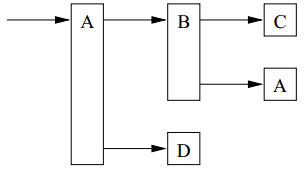
\includegraphics[width=\textwidth]{../images/06-DePauw-ExecutionPattern}
		\caption[Execution Pattern Notation by de Pauw et al.]{}
		\label{fig:NotationExecutionPattern}
	\end{subfigure}
	
	\caption[TOC Caption]{
		a) Functions-Instances-Matrix by de Pauw et al., adapted from \cite{de_pauw_visualizing_1993}.
		
		b) Execution Pattern Notation by de Pauw et al., taken from \cite{de_pauw_execution_1998}.
	}
	\label{fig:ObjectInteractions}
\end{figure}

\textsc{Scene} by Koskimies and Mössenböck \cite{koskimies_scene:_1996} provides interactive visualizations of Oberon programs in the form of scenario diagrams.
Execution traces from instrumented program runs serve as a basis, whereby the instrumentation can be conducted at the granularity of Oberon modules.
Just like in UML sequence diagrams, objects are represented by vertical lines, and interactions between those objects are represented by horizontal arrows.
To deal with the problem of large traces and limited screen  real estate, the authors propose \emph{call compression} and \emph{partitioning}.
Call compression means that all message sends are collapsed initially and can be expanded by the user through clicking on them.
Partitioning is employed since the authors consider vertical scrolling as acceptable, but want to avoid horizontal scrolling. Thus, if the size of the diagram exceeds the horizontal viewport, a new window is opened and the visualization is continued there.
\textsc{Scene} also allows the user to inspect the state of an object before and after a method invocation.
However, contrary to our approach which displays the actual state of objects and allows the user to explore complex referenced objects, this feature only utilizes user-provided \emph{Print} methods every object is supposed to have and displays static print strings.
\textsc{Scene} also does not offer ways to filter a trace by methods or classes or to search for specific entities of interest.

Lange and Nakamura present \textsc{Program Explorer} in the context of design pattern based framework understanding \cite{lange_interactive_1995, lange_program_1995, lange_object-oriented_1997}.
Based on the assumption that the combination of abstract concepts like classes and their relationships and the concrete objects and their interactions is the fundamental requirement to the understanding of object oriented systems, \textsc{Program Explorer} offers class inheritance views, object graphs and interaction charts.
Contrary to our approach, object state exploration is not supported.
To ensure a certain degree of scalability of the information presentation, \emph{view navigation} and \emph{integration} are provided.
Within a given view, \emph{navigation} can be used to explore the presented information interactively, starting from an initial focus point and going to regions of further interest.
\emph{Integration} enables the user to transfer a defined focus between different views.
Both concepts are similar to the navigation through a scenario offered by \textsc{PathObjects} and the bidirectional connection to the static view provided by \textsc{PathView}.
To reduce the size of the traces that are generated from instrumented executions of C++ programs, \textsc{Program Explorer} also supports \emph{trace localization}, which means that classes of interest can be selected through the instrumentation GUI and only selected classes will be instrumented.
As compared to \textsc{PathObjects}, the latter offers a more fine-grained approach through the selection of methods of interest, instead of solely filtering by classes.

The unique feature of \textsc{ISVis} \cite{jerding_using_1997} that also presents object interactions in the form of sequence diagram-like scenario views is the concept of \emph{ information murals} \cite{jerding_information_1998, jerding_visualizing_1996}.
The target of this approach is to provide a miniature view of large execution traces as a whole (cf. Figure \ref{fig:NotationMural}).
Classes are represented by rows on the vertical axis and a message between objects of different classes is drawn as a vertical line between the respective rows.
Users can assign colors to classes of special interest, which leads to an emphasis of the corresponding messages.
The horizontal axis represents time.
To avoid over-plotting, Visual properties like gray-scale shading or color intensity are exploited to map multiple elements to a single pixel or column.
Thus, the visual properties an original visualization would have if it could be viewed in its entirety are supposed to be preserved as effectively as possible.
Jerding et al. state that this view enables the user to find interaction patterns in large execution traces, which again helps in identifying usage scenarios and program components.
However, contrary to the timeline offered by \textsc{PathObjects}, murals appear to be unsuitable for the mapping of additional metrics to the various dimensions of the individual elements.

\begin{figure}[tb]
	\centering
	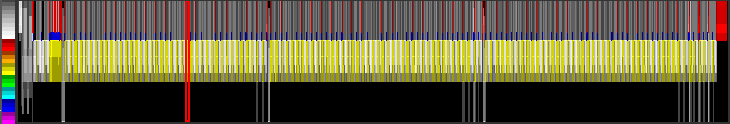
\includegraphics[width=0.8\textwidth]{../images/06-Mural}
	\caption[Information Mural by Jerding et al.]{Information mural displaying the execution of a bubble-sort algorithm with over 90,000 messages between 200 classes (adapted from \cite{jerding_information_1998}).}
	\label{fig:NotationMural}
\end{figure}

\textsc{Collaboration Browser} by Richner and Ducasse \cite{richner_using_2002} is a tool that focuses on the recovery of object collaborations and roles from dynamic information.
Since the process of automatic design recovery is said to yield poor results, the authors favor an iterative process steered by an engineer.
To facilitate such a process, \textsc{Collaboration Browser} offers two main features: \emph{pattern matching} and \emph{querying}. 
Typically, a user would first create collaboration patterns by defining pattern matching criteria, and then proceed by iteratively querying about patterns in which classes or methods of interest participate.
Finally, to understand a collaboration, an instance of a collaboration pattern can be visualized in the form of interaction diagrams, which are almost identical to UML sequence diagrams. \todo{compare to PathObjects}

Systä et al. present a reverse engineering environment called \textsc{Shimba} \cite{systa_shimba_2001}, which supports both static and dynamic analysis of Java software systems.
Static information about software entities like classes, interfaces and their relationships is extracted from the bytecode representation and visualized using \textsc{Rigi} \cite{muller_understanding_1993} in the form of directed dependency graphs.
Besides the computation of some of the metrics of Chidamber's and Kemerer's suite \cite{chidamber_metrics_1994}, \textsc{Rigi} also can be utilized to build abstractions, for instance by aggregating classes into their respective packages.
Runtime traces are collected with the help of a customized SDK debugger and can be synthesized as UML-like sequence and statechart diagrams through \textsc{SCED} \cite{koskimies_automated_1998,systa_understanding_2000}.
\textsc{Shimba} supports bidirectional model slicing between \textsc{Rigi} graphs and \textsc{SCED} diagrams.
On one side, \textsc{Rigi} can be used to restrict the amount of collected execution events through the selection of components of interest. Thus, the scope of the generated \textsc{SCED} diagrams is reduced.
On the other side, starting from a \textsc{SCED} diagram, static views covering the affected components can be obtained.

Similar to our approach, Cornelissen et al. propose the automated reconstruction of simplified UML sequence diagrams from test cases \cite{cornelissen_visualizing_2007}.
In order to keep the generated diagrams at a manageable size, the authors suggest and partially implement a number of abstraction and filtering techniques, many of which are also supported by \textsc{PathObjects}.
Among others, these are the definition of minimum and maximum stack depths (and the omission of method calls below and above those thresholds), filtering of constructors and calls of getters and setters, pattern recognition or object clustering.
However, the presented prototype is not interactive in the effect that users could step through the trace or collapse or expand nodes.
Object state exploration mechanisms are also unprovided for.
Cornelissen et al. evolved their approach into massive sequence and circular bundle views that are supposed to visualize much larger execution traces than those resulting from test cases \cite{cornelissen_understanding_2007, cornelissen_execution_2008}.

\section{Object-Centric Debugging}

\begin{figure}[b]
	\centering
	
	\begin{subfigure}[b]{0.45\textwidth}
		\centering
        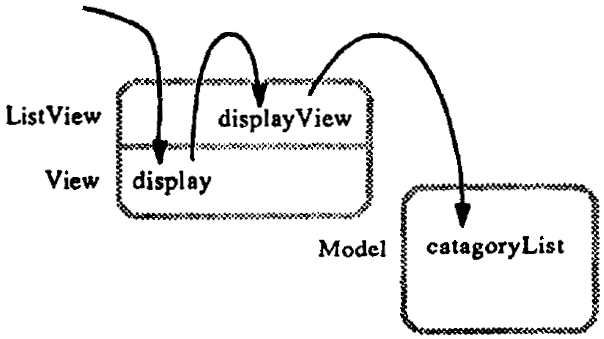
\includegraphics[width=\textwidth]{../images/06-Cunningham-Diagram}
        \caption[Object Interaction Diagrams by Cunningham and Beck]{}
		\label{fig:DebugCunningham}
	\end{subfigure}
	\quad
	\begin{subfigure}[b]{0.45\textwidth}
		\centering
		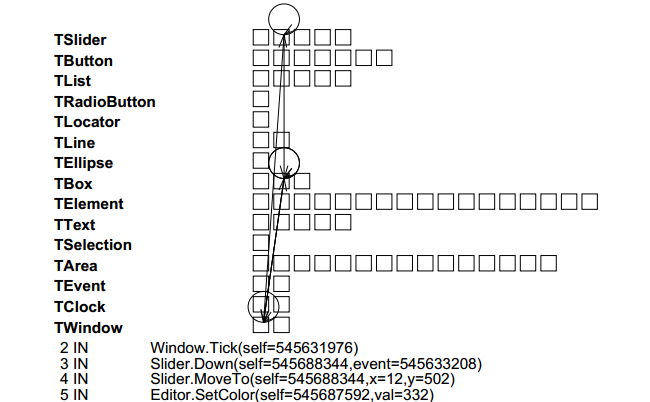
\includegraphics[width=\textwidth]{../images/06-Laffra-HotWire}
		\caption[Object Interaction View provided by \textsc{HotWire}]{}
		\label{fig:DebugLaffra}
	\end{subfigure}
	
	\caption[TOC Caption]{
		a) Cunningham's and Beck's notion of diagramming object interactions, taken from \cite{cunningham_diagram_1986}.
		b) Object interaction view provided by \textsc{HotWire}, adapted from \cite{laffra_hotwire:_1994}.
	}
	\label{fig:VisualDebuggers}
\end{figure}

Cunningham and Beck propose a syntax for diagramming the message sending dialogue between objects in object-oriented computations (see Figure \ref{fig:06-1-Cunningham}) \cite{cunningham_diagram_1986, beck_system_1989}.
Similar to \textsc{PathObjects}, objects are drawn as boxes and message sends are represented by directed arcs between them.
Unlike the notation used by \textsc{PathObjects}, the space inside the boxes is not used to model the object state, but to emphasize method overrides and calls to implementations of superclasses.
For that purpose, the class hierarchy is represented by layers in a box.
Since the authors regard overriding as the more important concept over inheritance, subclasses are placed above superclasses in these layers. 
To allow for the generation of such diagrams, an additional pane is added to the Smalltalk-80 debugger. 
Objects and messages are added to this diagram area when using the standard debugger commands \emph{step} and \emph{send}. 
However, as automatic layouting is not supported, objects have to be placed by the user manually. 
The authors state that the debugger extension helped them to understand complicated computations better, enabling them to fix a long standing bug in the Smalltalk core.

\textsc{HotWire} by Laffra and Malhota \cite{laffra_hotwire:_1994} is a visual debugger for C++ and Smalltalk that requires source code level instrumentation of the system under investigation.
It aims to be easily extensible and therefore provides a declarative script language to allow users to define their own custom visualizations.
In the context of this thesis, one of the predefined views that gives an overview of all objects in a system (cf. Figure \ref{fig:06-1-Laffra}) is of particular interest.
It groups instances according to their type, whereas each box in a line represents an instance of the class in the left column.
The bottom of the view shows the current call stack, including print strings of method arguments.
The top of the call stack is represented by arrows between instances, indicating which objects currently participate in the computation.
The authors also suggest to use different levels of color saturation to indicate how often specific instances receive messages and thus to visualize how the work is distributed across different objects.
In contrast to \textsc{PathObjects}, \textsc{HotWire} does not include mechanisms to exclude irrelevant objects or messages from the visualization.
It also does not provide means to find points in the execution history where specific objects or messages are involved.

Ressia et al. try to close the gap between the static nature of traditional  debugging with breakpoints, and the questions developers ask during debugging,  which often focus on specific individual objects \cite{ressia_object-centric_2012}.
In addition to conventional breakpoints that refer to static source code entities, their approach which they call \emph{Object-Centric Debugging} allows to specify new kinds of breakpoints with reference to particular objects.
\todo{wdh} This allows the developer to specify breakpoints on an already running program on two dimensions of object oriented computations.
The first dimension is related to object state and state changes.
For that purpose, the authors introduce \emph{halt on write} and \emph{halt on read} breakpoints that can be defined on instance variables of specific objects.
The second dimension covers the interaction of objects and includes, among others, \emph{halt on call}, \emph{halt on invoke} or \emph{halt on interaction}.
To allow for the definition of such breakpoints, the authors extended the Pharo Smalltalk debugger and inspector in their prototypic implementation.
That means that the approach is still heavily based on the execution stack visualization of traditional debuggers and does not offer any new or additional visualizations.
However, it is still supposed to reduce the time required for debugging notably and thus to speed up the understanding of object interactions.

Lencevicius et al. propose a declarative query language that is supposed to help in the debugging of object-oriented programs \cite{lencevicius_query-based_1997, guerraoui_dynamic_1999}.
Their queries consist of a definition of the search domain (similarly to a selection of types of interest) and a number of constraints on arbitrary fields of the objects of this domain.
Consequently, the result of such a query is a collection of objects from the search domain that match the given constraints.
Thus, questions like "\textit{which objects have a reference on a given object}" or "\textit{which user interface elements are currently visible in a given container}" can be answered.
However, since the queries are executed against specific system snapshots during a debugging session, they can not be used to investigate actual object interactions.
For instance, it is impossible to formulate queries about message sends (like "\textit{which objects send or receive s specific message}" or "\textit{to which objects does a given object send messages}".
\textsc{PathObjects} provides answers to such questions either visually or through the integrated search engine.

\section{Object-Oriented Learning Environments}
\textsc{JAVAVIS} by Oechsle and Schmitt \cite{diehl_javavis:_2002} was designed to aid in the teaching of the object oriented programming concepts of the Java environment.
It utilizes the Java Debug Interface to retrieve run-time information and can be used to step through the execution of a program.
Two main views are offered.
First, an UML sequence diagram is used to display the function call history of the current execution which grows successively as the user steps through the program.
Second, an UML object diagram is generated for each active invocation on all call stacks of the program under investigation.
These diagrams display the state of the receiving object, of local variables, and of the method's arguments.
That means that contrary to the approach implemented by \textsc{PathObjects}, object state and communication between objects are presented in different views.
The choice of using JDI debug sessions as data source implies further restrictions.
Only those objects that are currently present on the call stack can be inspected, while our solution also allows the user to explore the state of objects that have been used in the past but are not involved in the computation that is displayed.
Furthermore, a search for object or method occurrences is not possible for the future execution, and also not offered for the execution history.
The same applies to the unrestricted navigation to specific points of the execution.

\todo[inline]{Blue/BlueJ ?}
\todo[inline]{jGrasp?}
\todo[inline]{Jeliot}